\documentclass{sigchi}

\toappear{}
\pagenumbering{arabic}

% Load basic packages
\usepackage{balance}
\usepackage{graphics}
\usepackage[T1]{fontenc}
\usepackage{txfonts}
\usepackage{times}
\usepackage{url}
\usepackage{color}
\usepackage{textcomp}
\usepackage{booktabs}
\usepackage{ccicons}
\usepackage{todonotes}
\usepackage[pdftex]{hyperref}

% llt: Define a global style for URLs, rather that the default one
\makeatletter
\def\url@leostyle{%
  \@ifundefined{selectfont}{\def\UrlFont{\sf}}{\def\UrlFont{\small\bf\ttfamily}}}
\makeatother
\urlstyle{leo}

% To make various LaTeX processors do the right thing with page size.
\def\pprw{8.5in}
\def\pprh{11in}
\special{papersize=\pprw,\pprh}
\setlength{\paperwidth}{\pprw}
\setlength{\paperheight}{\pprh}
\setlength{\pdfpagewidth}{\pprw}
\setlength{\pdfpageheight}{\pprh}

% Make sure hyperref comes last of your loaded packages, to give it a
% fighting chance of not being over-written, since its job is to
% redefine many LaTeX commands.
\definecolor{linkColor}{RGB}{6,125,233}
\hypersetup{%
  pdftitle={SIGCHI Conference Proceedings Format},
  pdfauthor={LaTeX},
  pdfkeywords={SIGCHI, proceedings, archival format},
  bookmarksnumbered,
  pdfstartview={FitH},
  colorlinks,
  citecolor=black,
  filecolor=black,
  linkcolor=black,
  urlcolor=linkColor,
  breaklinks=true,
}

\newcommand\Peter[1]{{\color{red}#1}}	% Assigns macro to text color
\newcommand\Ben[1]{{\color{blue}#1}}	% Assigns macro to text color

% create a shortcut to typeset table headings
% \newcommand\tabhead[1]{\small\textbf{#1}}

% End of preamble. Here it comes the document.
\begin{document}

\title{Interactive Exploration of the Employment Situation Report: From Fixed Tables to Dynamic Discovery.}

% \numberofauthors{4}
% \author{%
%   \alignauthor{Benjamin Bengfort\\
%     \affaddr{University of Maryland}\\
%     \email{bengfort@cs.umd.edu}}\\
%   \alignauthor{Xintong Han\\
%     \affaddr{University of Maryland}\\
%     \email{hixintonghan@gmail.com}}\\
%   \alignauthor{Assaf Magen\\
%     \affaddr{University of Maryland}\\
%     \email{amagen@umd.edu}}\\
%   \alignauthor{Hao Zhou\\
%     \affaddr{University of Maryland}\\
%     \email{zhhoper@gmail.com}}\\
% }

\numberofauthors{3}
\author{%
  \alignauthor{Benjamin Bengfort\\
    \affaddr{University of Maryland}\\
    \email{bengfort@cs.umd.edu}}\\
  \alignauthor{Peter Mancini\\
    \affaddr{University of Maryland}\\
    \email{pmancini@umd.edu}}\\
  \alignauthor{Ben Shneiderman\\
    \affaddr{University of Maryland}\\
    \email{ben@cs.umd.edu}}\\
}

\maketitle

\begin{abstract}

The Bureau of Labor Statistics (BLS) has provided the world with the United States' economic statistical data for decades, most notably in the form of the \textit{Employment Situation Report}. This report is a monthly news release by the Bureau of Labor Statistics that describes the results of the Current Population Survey \cite{_employment_2015}. Its release is widely anticipated by economists, journalists, and politicians as it is used to forecast the economic condition of the United States by describing ongoing trends and has a broad impact on public and corporate economic confidence. However, the online accessibility of this data is becoming quickly outdated. The report itself is in a PDF format that is comprised primarily of text and tabular information. Quickly and correctly interpreting the contents of the report is vital for quality reporting and decision making, but presently the report is more suited for longer study than deriving immediate insights. This work presents two prototype applications that utilize visual analysis methodologies to transform data in fixed tables to provide dynamic discoveries through visual interaction.


%This is done via a hierarchical tree structure that enables the user to explore a very large dataset in one interactive window. Usability studies generated positive results from users, who greatly favored BLSVisualizer over the traditional format for retrieving data.

\end{abstract}

\keywords{
	Bureau of Labor Statistics; Employment Situation Report; Information Visualization; Visual Analytics; Dashboard; D3; Data Science Pipeline; Tree Structure
}


\section{Introduction}

Since 1984, the Bureau of Labor Statistics (BLS) has served as the principal Federal agency responsible for measuring labor market activity, working conditions, and price changes in the economy. Data collected by the BLS can be sorted into four categories: Prices (e.g. Consumer Price Index, CPI), employment and unemployment, compensation and working conditions, and productivity. This data is collected via surveys designed by economists and statisticians to acquire information regarding demographic and industrial statistics, which are then released in a report to the public.

Results of the surveys are compiled in the \textit{Employment Situation Report}. This critical, monthly assessment of the state of labor in the United States is released by the Bureau of Labor Statistics (BLS) at 8:30 AM on the first Friday of the month. The ``Jobs Report'', as it's popularly called, is based on the Current Population Survey, which surveys individual households and the Current Employment Statistics Survey, which surveys employers. Together, these two surveys give a snapshot view of the number of employed and unemployed Americans, how many hours they are working, and a variety of other facts and figures. In recent years, this report has been used to measure economic and political solutions to the 2008 downturn, as well as the performance of politicians themselves. As a result, news media widely publicizes the upcoming release of the report each month and follows the publication with widespread analyses and critiques. Perhaps thanks to its publicity, the report is more recently being used as a forecasting tool by firms on Wall Street, largely because the report is an indicator of investor and employer confidence in the growth of the economy \cite{mahorney_what_2013}.

The report is delivered on the BLS website in both PDF and HTML format, comprised mostly of text and tabular information and is well suited for deep study rather than rapid analysis. Because of the report's forecasting power and journalistic impact, fast and correct interpretation of the report's information is essential; however, the current format does not lend itself well to the quick derivation of insights. Moreover, the report is not as easily accessible to a general audience, favoring economic language and measurements. A visual analytics methodology \cite{keim_mastering_2010} using information visualization techniques would benefit the \textit{Employment Situation Report}, allowing for fast, correct interpretation of the current employment situation in the United States, as well as making the report more generally accessible.

In order to assess the quality and user friendliness of their website, the BLS, characteristically, conducts a survey on customer satisfaction. Figure \ref{CustSat} provides the customer satisfaction results from July 1, 2009 - June, 30 2011. The average satisfaction level was 75, which implies that the website has considerable room for improvement. The present work aims to increase customer satisfaction and provide a more enjoyable experience for the data-seeking users. The purpose of this work is to gather data contained in thousands of tables and present it in such a manner that is easily navigable and provides the user with an immediate visual representation of the dataset.

The tools presented here were developed with the intent of being easy to use, visually clear products with a powerful capability to evoke insights from the user based on the presented data. From a design standpoint, it is the designers job to manipulate the perception, cognition, and communicative intent of a visualization \cite{agrawala2011design} by understanding the principles of what makes a good design. Producing a ``friendly data graphic'' \cite{tufte1983visual} requires the designers to include a balance of useful features while also remaining aesthetically pleasing and not overwhelming to the user. Concepts such as color \cite{macdonald1999using}, font \cite{moere2011role}, and transitions \cite{heer2007animated} have been shown to affect usability of a visualization and have been strategically considered in the present work.

The combination of computer analytical processes with the human ability to quickly understand patterns leads to a reasoning system of discovery through interaction \cite{green_visual_2008}. This work focuses on compiling and arranging the tabular BLS data into an easily navigable, user-friendly interface that allows the user to see trends in the data, from which to potentially draw immediate insights. The goal of these interactive visualization tools is to significantly improve the user interface of the current BLS website and benefit the entire labor statistics community

\begin{figure}[t]
    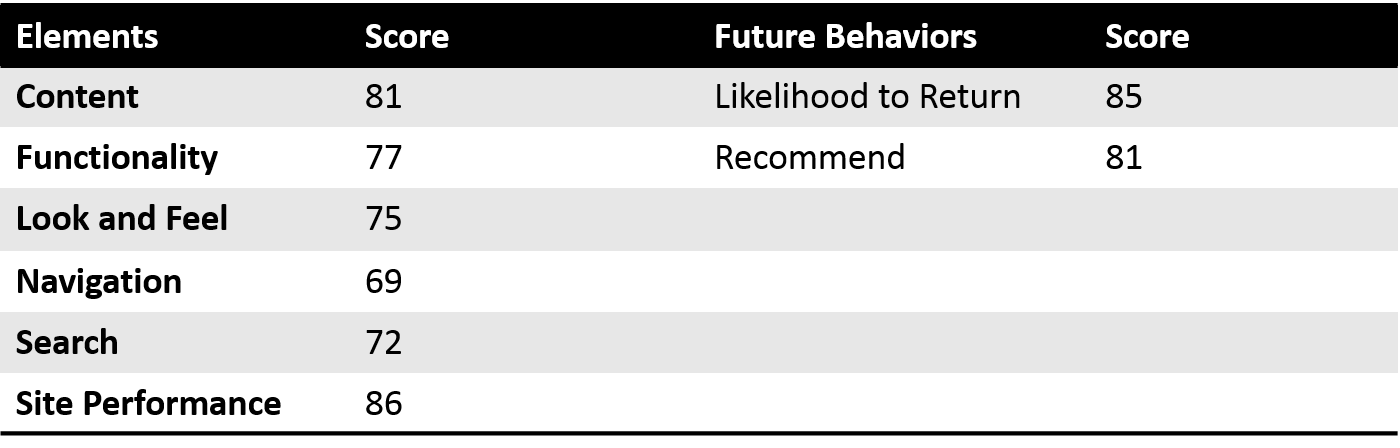
\includegraphics[width = 3.5in]{figures/BLSSurvey_ppt.png}
    \caption{BLS customer satisfaction survey for July, 1 2009 - June, 30 2011.}
    \label{CustSat}
\end{figure}

\section{The BLS Data Pipeline}

The Jobs Report is released monthly based primarily on two national surveys: the Current Population Survey and the Current Employment Statistics survey. Data was also ingested from state and metropolitan surveys: the Local Area Unemployment Statistics survey and Current Employment Statistics for State and Metropolitan economic divisions. Using these data sources created a unique challenge for a visual analytics data product - the system had to be able to adapt and acquire new information automatically, and to display important headlines on demand.

Our initial architecture therefore relied on the pedagogical model of the ``data science pipeline'' as described in \cite{ojeda_practical_2014}. The data science pipeline is an analytical framework, describing preparatory analytical steps of ingestion, wrangling, storage, and pre-computation. We replaced inferential and modeling statistical methodologies with a visual analysis methodology. The resulting ``BLS Data Pipeline'' is described by Figure~\ref{fig:pipline}. The ingestion component utilized the BLS API to download individual time series, which then had to be wrangled to normalize the data and input missing values for storage. Initial computations were then run on the data set to generate other data sources (for example a rate of change data set was computed on each time series). The data storage then powered an interactive API that was utilized by our visual front-end.

\begin{figure}[!h]
    \centering
    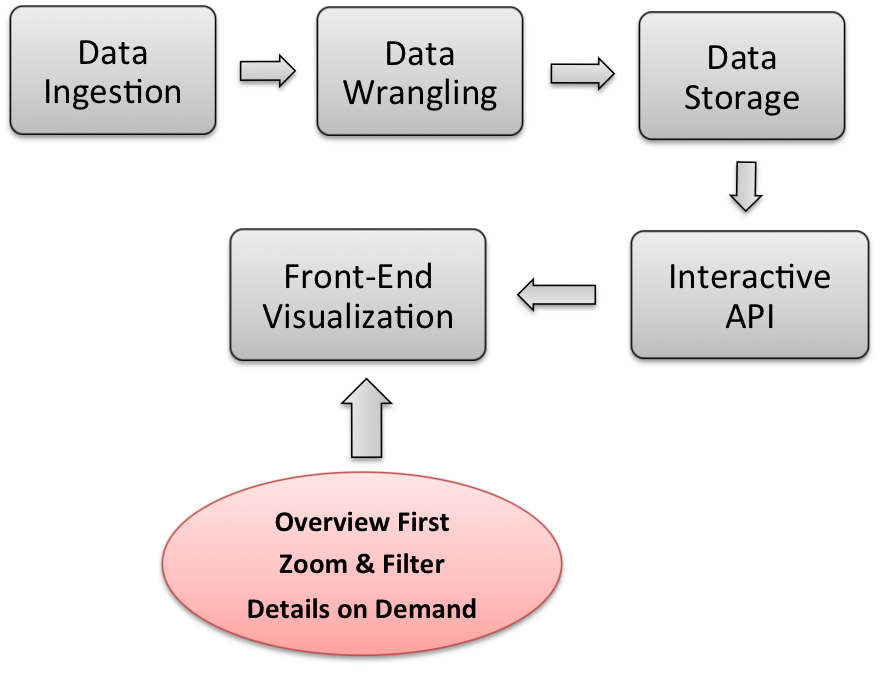
\includegraphics[width=0.9\columnwidth]{figures/pipeline.png}
    \caption{The BLS data pipeline, a model for combining monthly data ingestion with a visual analytics workflow.}~\label{fig:pipline}
\end{figure}

This section will briefly cover the data sources used in our project, as well as the associated architecture of our implementation.

\subsection{Data Sources}

The Bureau of Labor Statistics provides a large amount of data gathered by surveys conducted by various organizations of the United States Department of Labor. Three independent surveys: the Current Population Survey, the Current Employment Statistics survey, and the Local Area Unemployment Statistics survey provide the majority of information that is used in our application to explore the employment situation of the United States at both the national and state levels. Each of these data sources adds dimensions to a variety of visual analyses, and when contextualized together provides the best possible opportunity for insight discovery.

The primary data source for the Jobs Report is the Current Population Survey (CPS) \cite{_labor_????}, which is a monthly survey of households. This survey focuses on the relationship between demographics and employment and, at the national scale, provides a comprehensive data set on the labor force, unemployment, earnings, hours of work, and other labor characteristics. It is in this survey that demographic statistics like gender, age, education level, or ethnicity are gathered.

A secondary source for the Jobs report, the Current Employment Statistics survey (CES) surveys employers rather than households for labor force information \cite{_current_2015}. The CES survey is not only national, but also provides granular data for state and metropolitan geographies as well. In our application we diffrentiate between national and local CES surveys with the acronyms CES and CESSM, respectively. This survey focuses on industry-specific details of employment, hours, payroll, and earnings and is useful as a classification for different labor categories rather than demographics.

Finally, the Local Area Unemployment Statistics survey (LAUS) fills in local regional information that relates demographic information to employment where the CPS only describes the national level \cite{_local_2015}. LAUS provides monthly employment, unemployment, and labor force data by census divisions that include states, counties, metropolitan areas, and many cities. Because LAUS is a household survey (by place of residence) the employment characteristics can give a much more focused view of how demographic trends influence employment and the local level.

Finally, datasets can be grouped by a variety of dimensions. The employment dimensions include ``employment'', ``unemployment'', ``unemployment rate'', and ``labor force''. CES dimensions included industry descriptions like ``Mining and Construction'', whereas CPS and LAUS focused on demographic dimensions like age, gender, ethnicity, or level of education. Geographic dimensions had to be included for the CESSM and LAUS data sets, ordered by both U.S. Census economic divisions as well as by state.

\subsection{Data Ingestion}

The Bureau of Labor statistics provides two public data APIs that use RESTful state transfer mechanisms to deliver data on demand to users for particular time series information in various BLS programs. The APIs accept HTTP requests for information to URL endpoints that describe the required resource, then return information in paginated JSON format. We used the Version 2.0 implementation of the BLS API, which requires registration to obtain an API key. Such registration allows BLS to better understand what applications are using its data, but also allows developers more flexible access to the BLS data source.

We created a Python tool for downloading BLS data by providing a list of BLS IDs for each time series. There are three primary ways of ingesting time series: by downloading a single source or multiple sources to an endpoint that only allows downloading of data for the past three years, or by using the registration endpoint to specify the start and end years for ingesting multiple time series. We ingested data for the current millennium: from January, 2000 to February, 2015, obtaining over 305,445 records from 1,684 time series. To obtain a list of time series to target our downloads, we wrote a web scraper which scraped the ``most popular'' pages from the BLS website itself.

\subsection{Data Wrangling and Storage}

Data from the BLS website is returned in a JSON format. However, each data source from individual surveys may be formulated differently. Data wrangling efforts primarily dealt with inputing missing data (from years where surveys were not collected) and correcting mistakes in the ingestion process (e.g. mislabeled series information). Data type conversion was also required as JSON is a string format. The result of the wrangling process was a normalized, relational data set that could be stored in a PostgreSQL database management system.

The data wrangling system also computed ``extra'' data sources that we thought might be interesting to the front end visualization. One of the primary extra sources was to compute the percent rate of change of a surveyed category. It was our hope that by including pre-computed data sets such as these, the visual exploration mechanism could combine both human and computer analytical efforts.

Data wrangling also involved our initial data exploration efforts. We discovered that in order to power our geographic analyses, we needed some sort of regional information (e.g. FIPS identification codes or larger economic areas). The BLS website, while providing information particularly related to a time series, provided no \textit{meta information} about the data source, which required data retrieved from other sources. For example, although we might download a time series entitled ``Tennessee, Professional and Business Services, Not seasonally adjusted - labor force'' - we still had to do the work of assigning the Tennessee FIPS code, 42, and to parse out whether or not the data set was seasonally adjusted, what dataset it related to (labor force) and what its modifier was (Professional and Business Services). To do this for 1684 data sources, we needed an automated mechanism to parse time series names. The challenges of adapting the data straight from the BLS website took up over 80\% of our development effort, and perhaps highlights how vital a visual analysis tools is for this type and quantity of data.


\subsection{System Architecture}

The ingestion mechanism can be polled on a monthly basis to retrieve new information from the BLS API, keeping the application up to date for immediate use by journalists. The data backend then powers a RESTful API built using Python and the Flask framework that serves a front-end javascript single page application, which primarily uses D3 for visualization methodologies. Other notable implementation details can be found on the Github project page: \url{https://github.com/bbengfort/jobs-report/}, where we have made our system open source using the MIT license. The project itself is currently deployed on Heroku and can be accessed via \url{http://elmr.herokuapp.com/}. It is our intent that this project can be explored in detail by the scientific and data community.

\section{Dashboard Design}

\begin{figure*}[!ht]
    \centering
    \includegraphics[width=1.75\columnwidth]{figures/time_series_new_1.png}
    \caption{The time series explorer dashboard allows users to visualize multiple raw time series information in two different charts for ease of comparison with different data ranges. The year slider allows zooming and filtering by year. Finally, this dashboard attempts to add important headlines as listed by the Jobs Report.}
    \label{fig:time_series}
\end{figure*}

The data provided by BLS that powered our web application came in the form of time series data. Although each individual time series did not contain massive amounts of information (approximately 182 data points representing each month in this millenium), the number of time series themselves exceed the ability for a human to organize and digest the various information. In order to provide a visual mechanism of exploration and interactive reasoning, our design philosophy was that of a ``dashboard of visualizations'' where users could select appropriate visualizations, and interact with them though the ``overview first, zoom and filter, details on demand'' sense-making process. The primary filtering process involved time sliders to create windows of time to explore, as well as selectively choose which data to include in the visualizations.

We implemented four dashboards to explore these techniques, each in their own seperate tabs across the top of the application:

\begin{enumerate}
    \item \textbf{Time Series Explorer}: Explore and compare specific time series data sets in a dual-graph display.
    \item \textbf{Geographic Choropleth}: Explore time series according to their regional factors and influences, and how regions change over time.
    \item \textbf{Data Export Utility}: Other visualization tools might benefit from the ingestion and wrangling work we've undertaken. Data export allows users to use the data in their tool of choice.
\end{enumerate}

The visual analysis process requires a ``dashboard'' methodology - where a user can interactively control as many aspects of the visualization as possible, and where multiple visualizations are adapted simultaneously. Each tab described above is a dashboard with its own custom controls. The Time Series Explorer allows users to explore all of the available time series with two chart windows and filter and zoom by a range of years. It also provides a ``headline view'' which attempts to highlight key information, such as percent change over a selected time period. The Geography Choropleth allows users to explore regional information in the continental United States, while also filtering for percent change. Finally, a data export dashboard allows users to download specific data with filters applied so that they can manipulate the data in their favorite visualization tools.

\subsection{Time Series Explorer}

Figure~\ref{fig:time_series} provides a snapshot of our design for the time series dashboard. The primary focus of this dashboard is two vertically stacked time series graphs, which allow for a visualization of multiple datasets at once. This is especially helpful if the two quantities are of different dimensional units (e.g. population and unemployment rate) and could not otherwise be plotted together. In order to better describe the dashboard, we have divided it into six regions labeled A-F.

Region A shows four tab navigation bars which allow users to switch between the three dashboards. The tab display is consistent across all dashboards, and as more visualizations are added, more tabs can be added as well. If the list of tabs grows too long, in the future we intend to allow users to select tabs for a personalized display that gives them quick access to the dashboards they use most (for example, national reporters may be less interested in local employment statistics).

Region B contains an ``at-a-glance headline view'' and year slider control. The headline view is intended to be an eye-catching ``at-a-glance'' instant insight framework that is based heavily on the headline in the Employment Situation Report. The headline is tied to the two major pieces of information that are published at the top of the report - the unemployment rate and the number of non-farm jobs. The at-a-glance headline also displays important information regarding the amount of \textit{change} from the last period - a major piece of information that most users want to know. It is for this reason that these headlines have such a prominent place in our application.

The year slider control also shown in Region B is one of the primary mechanisms for zooming and filtering information for every dashboard in the app. The year range slider allows users to select a window of time periods within the available time span and to zoom the data into that range. Other dashboards have period selectors rather than ranges, which allows users to identify trends or data for a specific period.

Regions C and D contain the primary controls for the time series displays in regions E and F, respectively. For this application we have downloaded 1684 data sets, each of which can be displayed. The challenge is how to allow a user to select data sets of interest quickly. Although we considered using an autocomplete or search mechanism, our prototype implementation simply uses a grouped, auto complete dropdown as shown in Figure~\ref{fig:select}. This design follows ``prevent error'' rule in the Eight Golden Rules of User Interface Design \cite{shneiderman_eight_????} as users can only select the databases that are available through our drag-down menu.

\begin{figure}[h]
    \centering
    \includegraphics[width=0.9\columnwidth]{figures/select.png}
    \caption{In order to minimize error, users select BLS time series data sets through a grouped, alphabetized dropdown.}
    \label{fig:select}
\end{figure}


\subsection{Geography Choropleth}

\begin{figure*}[!ht]
    \centering
    \includegraphics[width=1.75\columnwidth]{figures/geography_new_1.png}
    \caption{The Geography Choropleth dashboard implements a chorpleth style heatmap on the AlbersUSA projection of the United States, particularly at the state and regional level. Users can control the data set and colors with the control bar, and select the time period to visualize with a slider.}
    \label{fig:Geography}
\end{figure*}

Our second visual dashboard focused particularly on regional and state visual analyses by implementing a highly interactive choropleth map of the United States using the AlbersUSA projection, as shown in Figure~\ref{fig:Geography}. The dominant feature of this dashboard is the choropleth map of the United States which is directly connected to a selectable dataset from either the CESSM or LAUS datasets. By interacting with the controls on the left, users can select the data set, whether or not to implement seasonal adjustments, choose to show the rate of change calculation, and even select the color map. A slider at the top of the visualization controls the year for the map.

This style map was our first design for the application, and we focused heavily on its implementation. However, we discovered that the datasets were heavily weighted towards the larger states of California and Texas, reducing the usability of a choropleth, which requires a color scale to be effective. We normalized the data set using "percent change" computations as described in the wrangling section. In this case users can explore the magnitude of change in a specific time series per state, which is much more effective in the choropleth setting.

Region C is designed for users to select and adapt the data set they want to visualize. A grouped, alphabetized drag-down menu is used for users to select a data source from either LAUS or CESSM. Two check boxes allow users to specify whether they want to show ``seasonally adjusted'' data and the other to specify whether to show the percentage of change of the data compared with the previous month. After users make changes to these two check boxes, they need to click on the ``Change Database'' button to refresh the map. To offer a bit of cosmetic freedom to the user, we provide several color scale options with which to plot the data. depending on the quantity plotted, the user may prefer a particular form of color scale, e.g. sequential, diverging, etc.

Region E is the main choropleth that displays the main continental United States as well as Alaska and Hawaii. The legend shows the color scale at the bottom left. If users hover over an individual state, a tooltip pops up with detailed information. Users can also click on a state to zoom in and see specific information about that state.

%\subsection{Wealth of Nations Dashboard}
%
%\begin{figure*}[!ht]
%    \centering
%    \includegraphics[width=1.75\columnwidth]{figures/wealth_new_1.png}
%    \caption{A four dimensional visualization inspired by the famous ``Wealth and Health of Nations'' visualization. This visualization attempts to minimize the regional sizing of the geographic choropleth by encoding data in five dimensions: the X and Y axis representing an labor force characteristic, color representing region, and size representing the state's employment level. Finally, a slider controls the time dimension.}
%    \label{fig:wealth}
%\end{figure*}
%
%Our final dashboard implements the ``Wealth and Health of Nations'' visualization that was made famous by Hans Rosling's 2006 TED Talk \cite{_wealth_????} and which demonstrates many interesting capabilities of D3. We implemented this visualization to show how multiple D3 visualizations from the gallery could easily be added to the dashboard, but also to show how different dimensions from similar data could be visualized differently. In this case, the use of a scatter plot design instead of a choropleth to describe regional information. The dashboard is broken into regions as shown in Figure~\ref{fig:wealth}.
%
%Region C is the main part of this dashboard which contains the scatter plot, which incodes data in 5 dimensions: $x$ and $y$ axes, color, raidus, and time. The $x$-axis represents the size of labor-force and the $y$-axis represents unemployment rate. Each dot represents a state and the radius of the dot represents the employment level of that state. Each state is colored according to their economic region (e.g. northeast, midwest, west, etc). Moreover, user can select the time point of the data by moving the mouse left and right in the time region. By hovering the mouse over the plate, the name of that state will be shown. This dashboard provides a easy way of exploring insights based on two or even more different dimensions of the data for all the states simultaneously.
%
%Region B does not appear in our original design. However, when we carried out our usability study, we found that many users complain about the difficulty to choose the time by just moving the mouse left and right on the time region, especially when users want to fix the time point and hover on the plate to show the name of the state. In order to fix this question raised in the study, the common year slider is added to the top, consistent with other slider designs.

\subsection{Data Export}

Finally, the last dashboard implements a data exporting feature. Although this utility is not a visual analysis tool, it is meant to cater to users who choose to use other software, such as Excel or Tableau, to perform their own analyses. The ingestion and wrangling of time series data is not difficult, but it is time consuming. By allowing users to directly export the data from our tool, we hope to increase the number of analyses available, and the insights that can be gained. Datasets are then downloaded in CSV or JSON format.

\subsection{Data Management}

Because the ingestion utility is real time and because we expect that the visual analysis dashboards will change over time, we have implemented an admin screen that gives users an at-a-glance look at the state of the system as shown in Figure~\ref{fig:admin}. We hope to convey in this page the effort it took to wrangle and gather the data, but also provide a means for interacting with the real time ingestion system. For example, an ingestion log shows when data was fetched from the BLS web site, as well as the magnitude of the ingestion process.

Other details include the current version of the application, and the timestamps of the updates or ingestions. The status bar gives a quick view of any required maintenance for the system. A GREEN status indicates that the app is within a month of the last ingestion, YELLOW indicates that the app is less than six months since ingestion, and RED indicates that the app has not been updated in over six months. Database records also indicate the state and size of the database.

By creating an open utility that shows the ingestion process and the state of the database, we hope to allow users to have transparency in our analytical and systems methodology so that collaborative efforts can improve the system. Along these lines, our software is open source on Github, with links to full documentation, agile development boards, API documentation, and more all in the drop down. In the future, we hope to allow direct administration from this page, by kicking off ingestion, or editing time series directly.

\begin{figure*}[!ht]
    \centering
    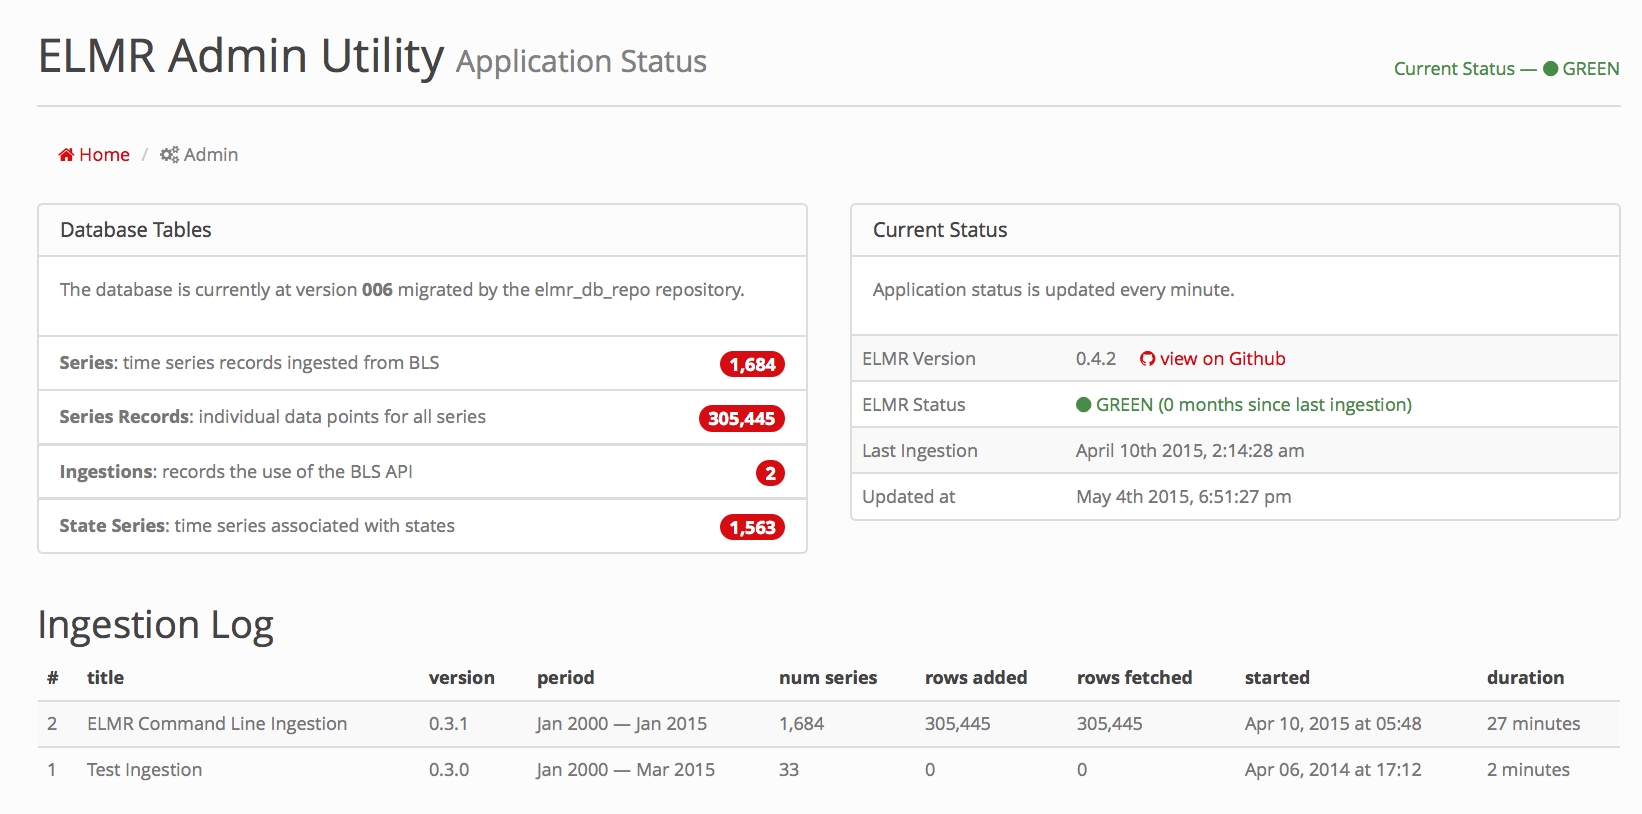
\includegraphics[width=1.75\columnwidth]{figures/Admin.png}
    \caption{Illustration of Admin resources.}
    \label{fig:admin}
\end{figure*}


\section{Hierarchical Navigation Design}

The dashboard applications presented in the previous sections provided a foundation from which to assess the strengths and weaknesses of visualizing the employment situation report. Through the iterative process of testing and redesign, the authors developed a second method for organizing and plotting the time series data.  A new tool, titled BLSVisualizer, was developed to allow users to clearly and interactively navigate through the employment data, which is conveniently organized in a hierarchical format.

The main feature of BLSVisualizer is the use of an interactive tree structure to obtain data. The tree structure is generated by implementing a parent-children hierarchy, from which the user can select his or her desired dataset. Much work has gone into studying the effectiveness of tree structures from both practical \cite{barlow2001comparison, plaisant2002spacetree} and aesthetic \cite{wetherell1979tidy, reingold1981tidier} standpoints. Barlow and Neville performed a parameter study on hierarchy visualizations by asking users to perform decision tree analyses on four different chart types: Organizational chart (or tree structure), icicle plot, tree ring, and treemap. Based on user response time and response accuracy, the authors concluded that the tree structure and icicle plots produced the most effective visualizations. The present study has considered the suggestions from previous work and decided to implement the hierarchical tree structure, due to its universal familiarity, ease of implementation, and aesthetic appeal.

The second feature of BLSVisualizer is the real-time drag-and-drop plot area, where the user can view the time series data in the form of two-dimensional line charts. While previously the user was forced to deal with hundreds of tables of data to simply compile a single time series, the user can now locate and plot the data quickly, ideally leading to more efficient data analysis.

Data was acquired via the API provided by the BLS in comma separated value (CSV) format. The CSV formatted data was converted to JSON format in order to more easily implement the hierarchical parent-child tree structure.

\begin{figure*}[t]
\centering
    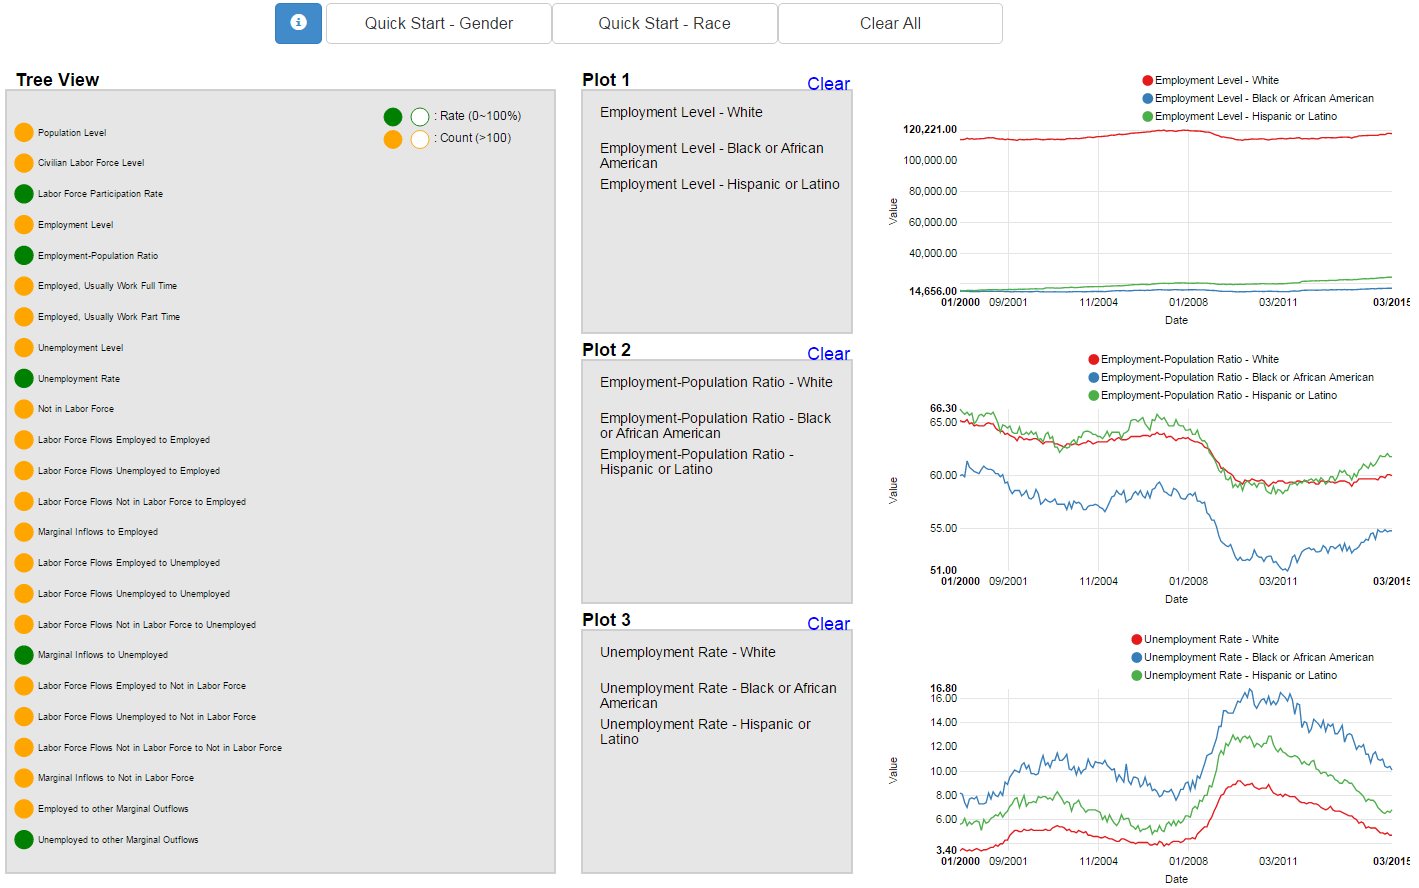
\includegraphics[width = 6.2in]{figures/BLSVisualizer.png}
    \caption{Example layout of BLSVisualizer }
    \label{BLSVLayout}
\end{figure*}

%The front-end interface utilizes primarily HyperText Markup Language (HTML), Cascading Style Sheets (CSS), and JavaScript. Javascript was largely employed via the Data Driven Documents (D3) library, from which most of the interactive displays were made.

\subsection{Tree Structure}

A primary step in any design process is to identify the design space. In this case, the space consists of multi-leveled categorical data. The nature of the design space lends itself to be organized in a hierarchical format. Hierarchies are typically displayed using a geometrically-transformed display \cite{keim2002information}. Such is done in the present work in the form of an interactively transforming tree structure, primarily written using the D3 library titled ``Collapsible Tree Layout''. The transitions are done in a smooth fashion that is aesthetically pleasing as well as visually effective.

Wetherell and Shannon \cite{wetherell1979tidy} provide a detailed description on what makes for an effective tree visualization. An important aspect of the analysis was the definition of three key \textit{aesthetics}. Each of their suggested aesthetics have been implemented into BLSVisualizer.

\begin{itemize}
\item \textit{Aesthetic 1}: Nodes of a tree at the same level should be along a straight line
\item \textit{Aesthetic 2}: Left and right children should remain left and right of the parent
\item \textit{Aesthetic 3}: Parent should be centered over its children
\end{itemize}

Another feature Wetherell suggested was to minimize the width of the tree as much as possible. However, the present authors and Reingold et al. \cite{reingold1981tidier} found this technique to cause a cluttered workspace and too narrow of a visualization.

**** This paragraph goes somewhere ****

%\Peter{This data was then organized into a pseudo-tree structure with labels denoting the level of the tree and and name of its category. For proper organizational purposes, the prefix of a child category was set to be the name of the parent category. Although, because the data was batch pulled from the BLS website and automatically sorted into the aforementioned hierarchical format, some of the data was sorted non-optimally. For example, several categories that should be grouped together as a ``parent'' result in several ``children'' with extensively long titles, e.g. two separate nodes ``Full time labor force looking for full time work - Men'' and ``Full time labor force looking for full time work - Women''. These two nodes can clearly be consolidated into a group ``Full time labor force looking for full time work'' with children for men and women. This issue can potentially be fixed by switching to a manual data importing and sorting process for BLSVisualizer; however, there are simply so many categories that this is likely unfeasible, or at least highly undesirable.  }

Most of the data, when exported from the BLS website, comes organized in a conveniently hierarchical manner. However, the authors further condensed some of the data to be organized in a more logical manner under more appropriate parent levels. To maintain a clutter-free environment, as the user expands the tree, only the bottom most levels are visible. To return to a previous level, the user can re-click on the last expanded parent and it will collapse the bottom level and return the previous level into view. The colors of each item correspond to either dimensional values (orange) or non-dimensional values (green), such as rates or percentages. Since this is a rather large dataset, this minor color coding will help the user more quickly identify the dataset he or she desires. The entire tree interface specifically complies with three of Shneiderman's Eight Golden Rules \cite{shneiderman_eight_????}: Strive for consistency, easy reversal of actions, and reduce short-term memory load.

\begin{figure}[t]
\centering
    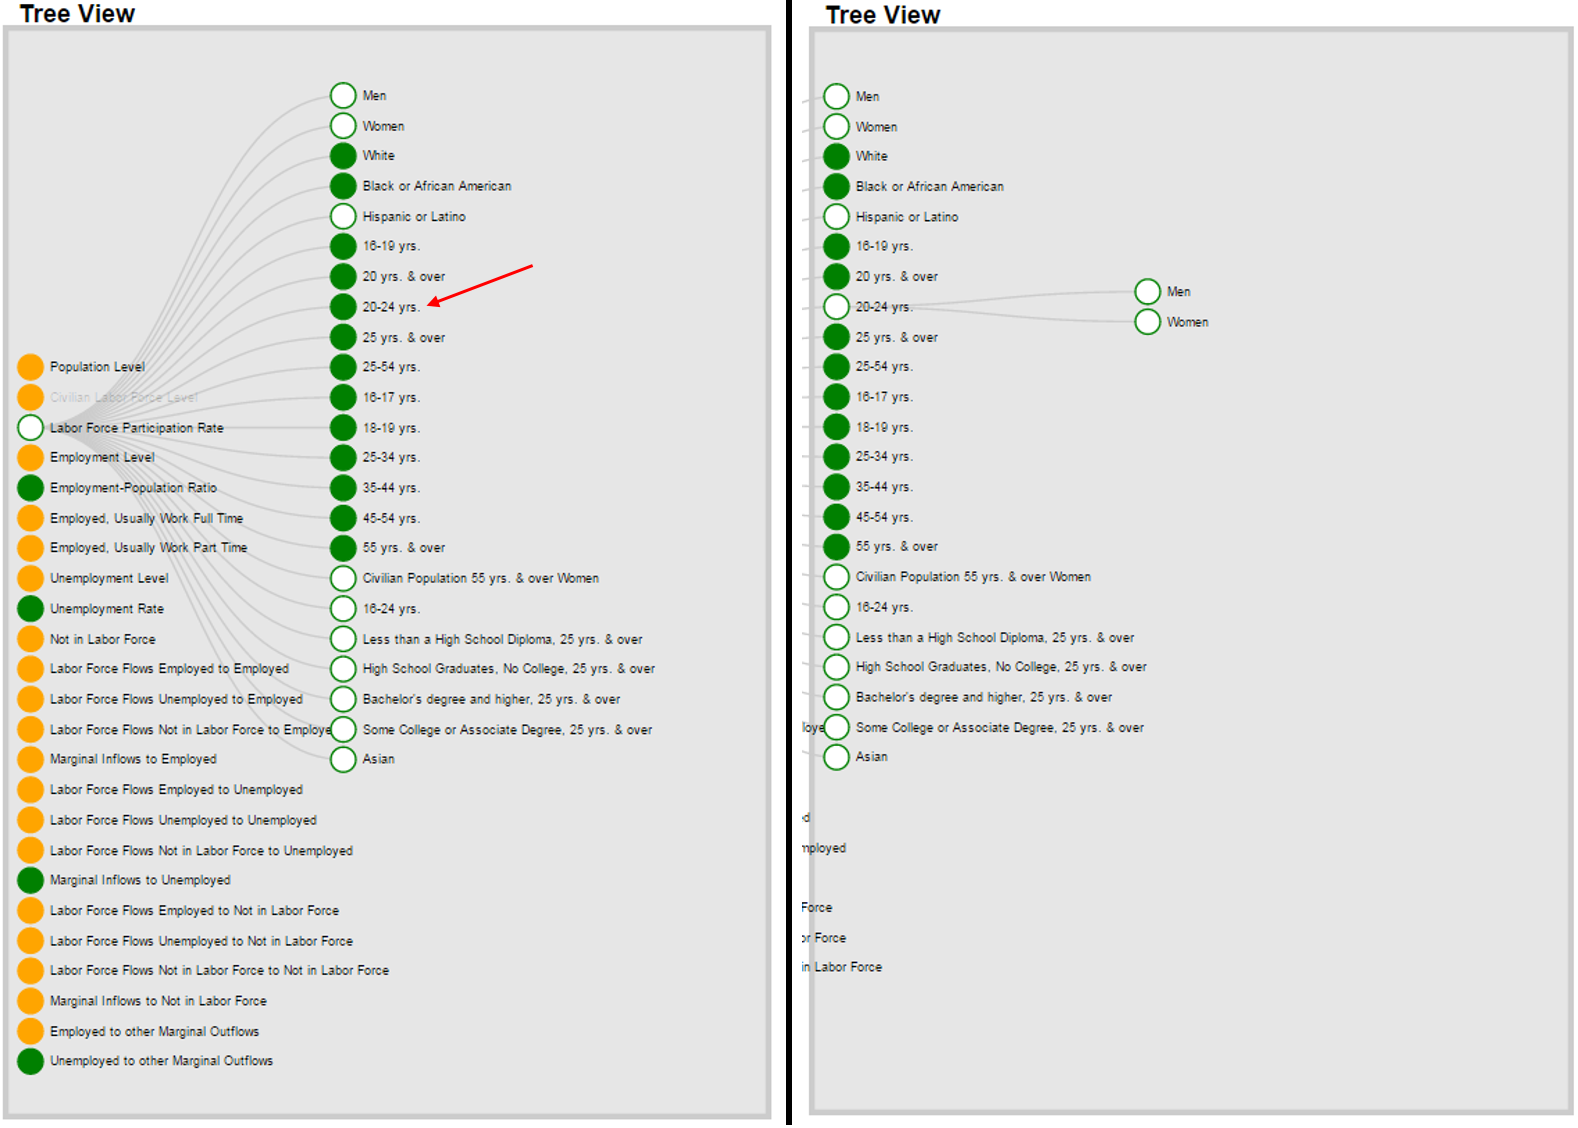
\includegraphics[width = 3.5in]{figures/tree2.png}
    \caption{Interactive hierarchical tree structure. (Left) One level into the hierarchy and (right) two levels into the hierarchy, during which the first level is pushed off-screen.}
    \label{TreeStructure}
\end{figure}

\subsection{Drag-and-Drop Plot}

To plot the time series data, the user may select a particular category and drag-and-drop that node into one of the middle boxes labeled ``Plot 1-3''. Each plot allows up to six items to be plotted at any one time. In order to preserve an easy reversal of actions, the user may simply click on the item in the plotting list to remove it from the chart. The ``clear'' button at the top of each plotting area provides a one-click option to clear the plot of all items. Again in compliance with the Eight Golden Rules, in order to ``prevent errors'' the application prevents the user from adding the same category more than once to the same chart.

\subsection{Chart Area}

The most important component of the visualization is the time series chart area. Dragging components into the center boxes causes the charts on the right to interactively update with the currently listed items. The nature of the time series data suggests that the shape of the graphic be a rectangular plot with the horizontal axis containing the date of each released BLS report. Line color was selected using the cartography tool ColorBrewer \cite{harrower2003colorbrewer}. This tool provided a very aesthetically pleasing array of six colors arranged with the intention of plotting data with qualitative differences. This is opposed to a quantitative color scale, e.g. light red to dark red, that would indicate the quantitative relationship between the items plotted. However, the two datasets of ``Employment Level - Men'' and ``Employment Level - Women'', for example, have no quantitative relationship. Thus, a color scale that provides significant contrast and legibility between the individual lines is ideal.

A popular mantra for designing an effective visualization is ``Overview first, zoom and filter, then details-on-demand'' \cite{shneiderman_eyes_1996}. BLSVisualizer, as a whole, does exactly that. The tree itself acts as an overview-to-zoom interactive element, allowing the user to dive deeper into the data, getting more detailed with each subsequent level. Additionally, the line charts, plotted from years 2000 to 2015 provide an overview in the sense that it is a line showing the trend of data over 15 years. However, upon hovering over the plot, a tooltip box will appear to provide the discrete monthly data points at the current location of the cursor. To help the user identify where along the x-axis the cursor is located, a vertical line spanning the height of the plot follows the cursor as it travels horizontally across the figure. The vertical position-indicator line is colored gray and is significantly thinner than the plotted time series data. The contrast in line weight represents a contrast in meaning, with the greater meaning given to the line with greater weight \cite{tufte1983visual}.

Figure \ref{TablePlot} provides a comparison of how the data is presented in both the current BLS website and in the BLSVisualizer. It is clearly shown that BLSVisualizer provides a service in terms of observational insightfulness when viewing the data that the current BLS website does not provide.

\begin{figure*}[t]
\centering
    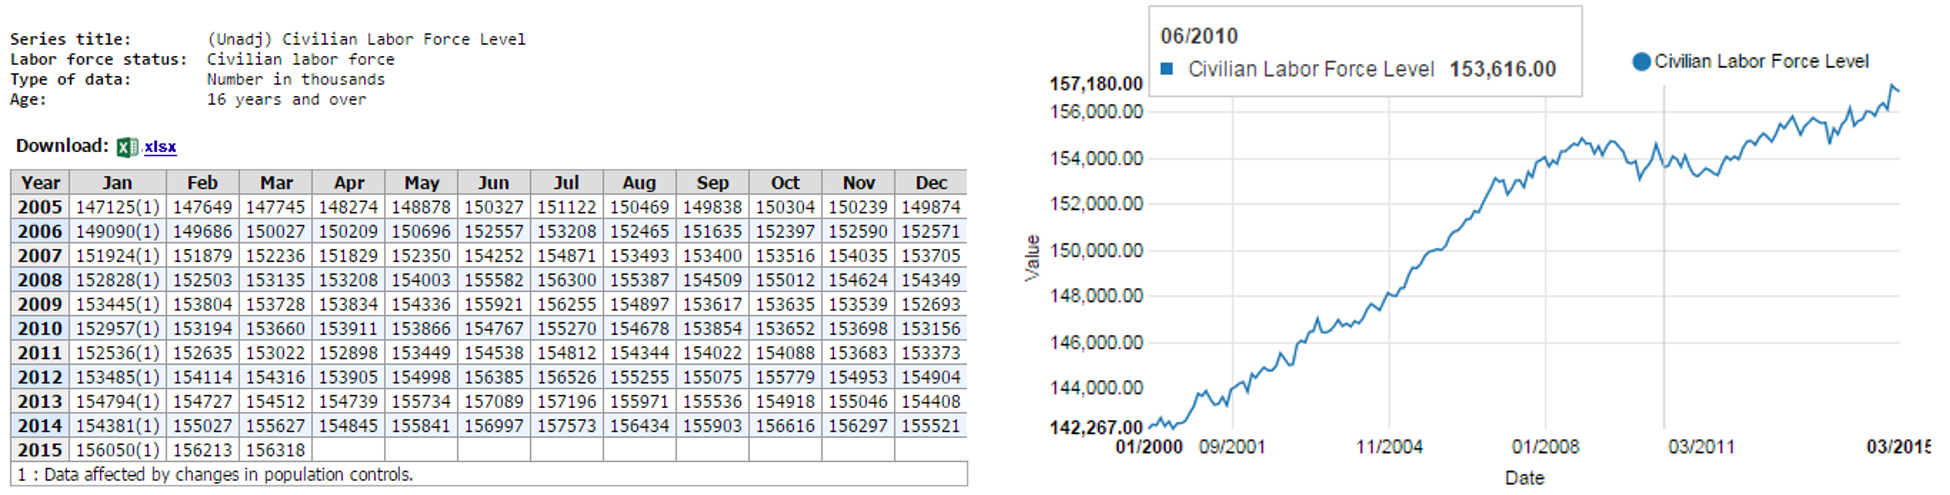
\includegraphics[width = 6.2in]{figures/PlotTable.png}
    \caption{Comparison of the two proposed sets of BLS data. (Left) Tabular data presently employed on the BLS website and (right) its equivalent visual counterpart presented in BLSVisualizer.}
    \label{TablePlot}
\end{figure*}


\subsection{Usability Study}

To examine BLSVisualizer and evaluate its potential as a visualization tool, the authors conducted remote and in-person usability tests with five users: all five were students, but only three participants had previous experience with visualization tools. Each test took about 5-10 minutes. Before starting the tasks section the authors collected basic information about the participants: age, gender, occupation, and experience with visualization tools.

The test was designed to progressively increase in difficulty, and went as follows:

\begin{enumerate}
  \item Create 3 graphs for the following categories:

\begin{itemize}
  \item Population level
  \item Employment level
  \item Marginal inflows to employment
\end{itemize}

  \item Change ``Unemployment level'' to ``Employment level''
  \item What was the white population level at 11/2011?
  \item Between 1/2008 to 1/2010, who had a larger increase in labor force flows from unemployment to employment: Men or Women?
  \item Compare, on the same graph, the effect of education level on unemployment rate.
  \item Compare the employment level of four different industries (both sexes).
\begin{itemize}
  \item Identify the largest industry (in terms of employment level) and compare the distribution of men and women for that industry.
\end{itemize}

\end{enumerate}

The first question simply asks the user to plot three separate datasets, which are all located on the first level of the tree, on the three chart areas. After reading the ``About'' section at the top of the page that describes how to use the tool, none of the users had an issue plotting the data. Two users brought up the fact that they were not aware that the ``About'' button was even an option. A clearer label would have remedied that issue.

The second question asked the user to remove one of the datasets they plotted and replace it with another. This question tests the ease of undoing an action, which is a very important feature in a visualization tool. Again, after locating the ``About'' pop-up window, all users were able to easily perform this task.

Question \#3 really tests the plausibility of replacing the current table look-up style of presenting the data with this interactive visualization. This task asked them to plot a time series and identify its value at a particular date (month/year). This task can be done in BLSVisualizer in two clicks, whereas on the BLS website it would likely take up to six clicks while visually sifting through dataset titles.

Question \#4 attempts to do what the current BLS data presentation cannot provide: Insights based on visualization of the data. The user is asked to identify a way to compare the effect of education level on unemployment rate. This question gave several users some trouble. They were not sure what exactly they were asked to do, but after exploring some of the categories and understanding what options they had to work with, all five users eventually produced the correct plot and drew the same conclusion. The conclusion was that the more educated you are the less likely you are to be unemployed.

The final task of the usability test asked the user to plot the employment level of four industries of their choice and identify the one with the highest level of employment. Once this dataset was located, they were asked to break that data down into a demographic study of male and female. This question was created to show the user that this visualization promotes breaking the data down into its parts to identify sources of a particular trend in the data. The users had minor difficulties with this task; however, once the task was completed, their comments conveyed that they were impressed with the overall utility of the tool.

The most frequent complaints about the BLSVisualizer interface were:

\begin{itemize}
  \item Lack of a Search bar
  \item Option to add plots
  \item Option to export data
  \item Font size was small
  \item Overlapping text for categories with long titles
\end{itemize}


\section{Conclusions and Future Work}

The present work focused on significantly improving the user interface of the current BLS website by compiling and arranging the tabular BLS data into an easily navigable, user-friendly interface with the intent of immediately identifying trends in the data and eliciting deeper insights. Our tool aggregates a large dataset of over a thousand time series, ingested using the BLS API on a monthly basis.

Initially, the authors created two primary dashboards: a Time Series explorer, where users can compare and contrast multiple time series through a stacked overlay, and a Geographic Choropleth map to investigate changes in employment according to demographics or industry at the state level. These dashboard applications, made primarily through the use of the D3 Javascript library,  provided a preliminary foundation from which to assess the viability of an interactive visualization for this particular dataet. Through iterative designs and usability tests, it was determined that visualization tools significantly improved the user experience. The authors then took the tool a step further and improved upon the time series application by introducing a hierarchical tree structure for more intuitive navigation. Additionally, a drag-and-drop method of plotting was introduced to give the user complete control over where the data was plotted and in what order. The chart area was also refined to provide discrete values at the point on the plot where the cursor is located to include on-demand detailed information to the user.

Usability tests of five users concluded that this application is significantly more useful, in terms of both finding the desired data and gathering conclusions based on trends. The usability testing also highlighted several areas of improvement for the visualization. The font and inter-category spacing will be made larger for improved legibility. Also, the ``Help/About'' sections will be more clear as to what capabilities the application has to offer. The most prominent user feedback, however, was the desire for a search bar to locate particular datasets.

This work provides a step in a positive direction toward which the BLS website can become a user-friendly, enjoyable tool, from which to observe the employment situation report. The applications presented here provide a base design from which to build upon, but the feedback and observations explained in this work should be considered when building more sophisticated tools to supplement the current BLS website.


\section{Acknowledgments}

This work was a team effort and many people collaborated on both the ELMR and BLSVisualizer projects. Would especially like to thank our classmates Bor-Chun Chen, Xintong Han, Jonggi Hong, Rotem Katzir, Assaf Magen, and Hao Zhou for all their support during the semester. Together they assisted us with software development, usability studies, and creating videos and demos. We would also like to thank those folks who participated in our usability study, and who critiqued our work to make it better.

We would also like to thank Jonathan Schwabish of the Urban Institute who provided the framework for the project, responded to emails, and gave us ideas. We would like to acknowledge the Bureau of Labor Statistics, particularly Emily Liddel and Tyrone Grandison who gave us guidance with the BLS API and specific information about the data sets being used. Finally, we'd also like to thank our professor, Ben Shneiderman, for being so enthusiastic about our project and helping create the opportunity for us to present at BLS.

\section{Links and Resources}

The following links contain more information relevant to the project as well as resources for further exploration (they have been shortened by the ter.ps URL shortner project for print format).

\begin{enumerate}
    \item ELMR Application: \url{http://ter.ps/985}
    \item Video Tutorial and Demo: \url{http://ter.ps/983}
    \item Github Repository: \url{http://ter.ps/984}
    \item Project Wiki: \url{http://ter.ps/986}
\end{enumerate}

\balance{}

% If you want to use smaller typesetting for the reference list,
% uncomment the following line:
% \small
\bibliographystyle{acm-sigchi}
\bibliography{paper}

\end{document}
